\documentclass[11pt,dvipdfmx]{jreport}
\usepackage{wuse_thesis}
\usepackage{indentfirst}
\usepackage{url}	% \url{}コマンド用.URLを表示する際に便利
\usepackage{graphicx}  % ←graphicx.styを用いてEPSを取り込む場合有効にする
\usepackage{listings,jvlisting} %日本語のコメントアウトをする場合jvlisting(もしくはjlisting)が必要

\usepackage{multirow}

\usepackage{color}

\renewcommand{\lstlistingname}{Program}
\newcommand{\todo}[1]{\colorbox{yellow}{{\bf TODO}:}{\color{red} {\textbf{[#1]}}}}
			% 他のパッケージ・スタイルを使う場合には適宜追加


%%%%%%%%%%%%%%%%%%%%%%%%%%%%%%%%%%%%%%%%%%%%%%%%%%%%%%%%%%%%%%%%%%%%%%%%

%%
%% 主に表紙を作成するための情報
%%

%%  タイトル(修論の場合は英語表記も指定)
\title{分散台帳を用いた農産物の認証と\\トレーサビリティ評価\\-有機農産物の認証におけるケーススタディ-}
%\etitle{Test\\Test\\Test}

%%  著者名(修論の場合は英語表記も指定)
\author{原口 拓也}
%\eauthor{Akinori Ihara}

%% 卒業論文・修士論文(以下のどちらかを選択)
\bachelar	% 卒業論文(4年生用)
%\master  	% 修士論文(M2用)

%%  学科・クラスタ
\department{システム工}
%\department{デザイン情報}
%\department{デザイン科学}

%%  学生番号
\studentid{60246233}

%%  卒業年度
\gyear{2023}		% 提出年が2022年なら,2021年度

%%  論文提出日
\date{2024年2月13日}	% 修士の場合は月(2021年2月)までとし,英語表記も指定
%\edate{February 2021}	% 修士の場合,こちら(英語表記)も有効化

%%%%%%%%%%%%%%%%%%%%%%%%%%%%%%%%%%%%%%%%%%%%%%%%%%%%%%%%%%%%%%%%%%%%%%%%

\begin{document}

\maketitle

%%
%%  概要
%%
\begin{abstract}
本研究では,農産物の認証とそのトレーサビリティについて,分散台帳を用いたシステム設計とその評価を提案し,有機農産物におけるケーススタディによってその課題と可能性に関して評価する.

 食品流通において,食の安全意識の高まり,持続可能性への関心から,食品生産の管理に対して,様々な認証制度が確立されてきた.その中でも日本農林規格(JAS)は,2000年(平成12年)に施行された改正JAS法に基づき,有機農産物やその加工食品に対して制定された.消費者はその認証制度によってその商品を選択する判断基準の1つとなっている.しかし,有機食品のトレーサビリティには有機ラベルの認証詐欺,食品情報の透明性への懸念などいくつかの問題が見受けられる.
 
  本研究では有機農産物の認証に関して,信頼性の観点,食品情報の透明性を向上することを目的とする.そのために複数のノードが同一のデータベースを持つことにより改ざん検出が容易なデータ構造を持つ分散台帳を用いたデジタル認証を有機JAS規格へ適用した.また,その認証システムを有機キウイを用いたケーススタディを行い,生産者,消費者の2者の視点から評価を行い,分散台帳を用いた農産物認証システムの可能性を提示する.

\end{abstract}

%%  目次
\tableofcontents

%%  図目次 (図目次をいれたければ以下のコメントをはずす)
%\listoffigures

%%  表目次 (表目次をいれたければ以下のコメントをはずす)
%\listoftables

\newpage
\pagenumbering{arabic}	% 以降のページ番号を算用数字に

%%%%%%%%%%%%%%%%%%%%%%%%%%%%%%%%%%%%%%%%%%%%%%%%%%%%%%%%%%%%%%%%%%%%%%%%

%%
%%  本文はここから
%%

\chapter{はじめに}
多くの消費者は食品を選択する際,食品の安全性を重視する.図\ref{fig:zyuusi}は農林水産省の「食品を選択する際に重視すること」~\footnote[1]{https://www.maff.go.jp/j/syokuiku/ishiki/h29/zuhyou/z2-6.html}を示す.この調査結果では,安全性を重視する消費者は55.7%となっている.
\begin{figure*}[t]
	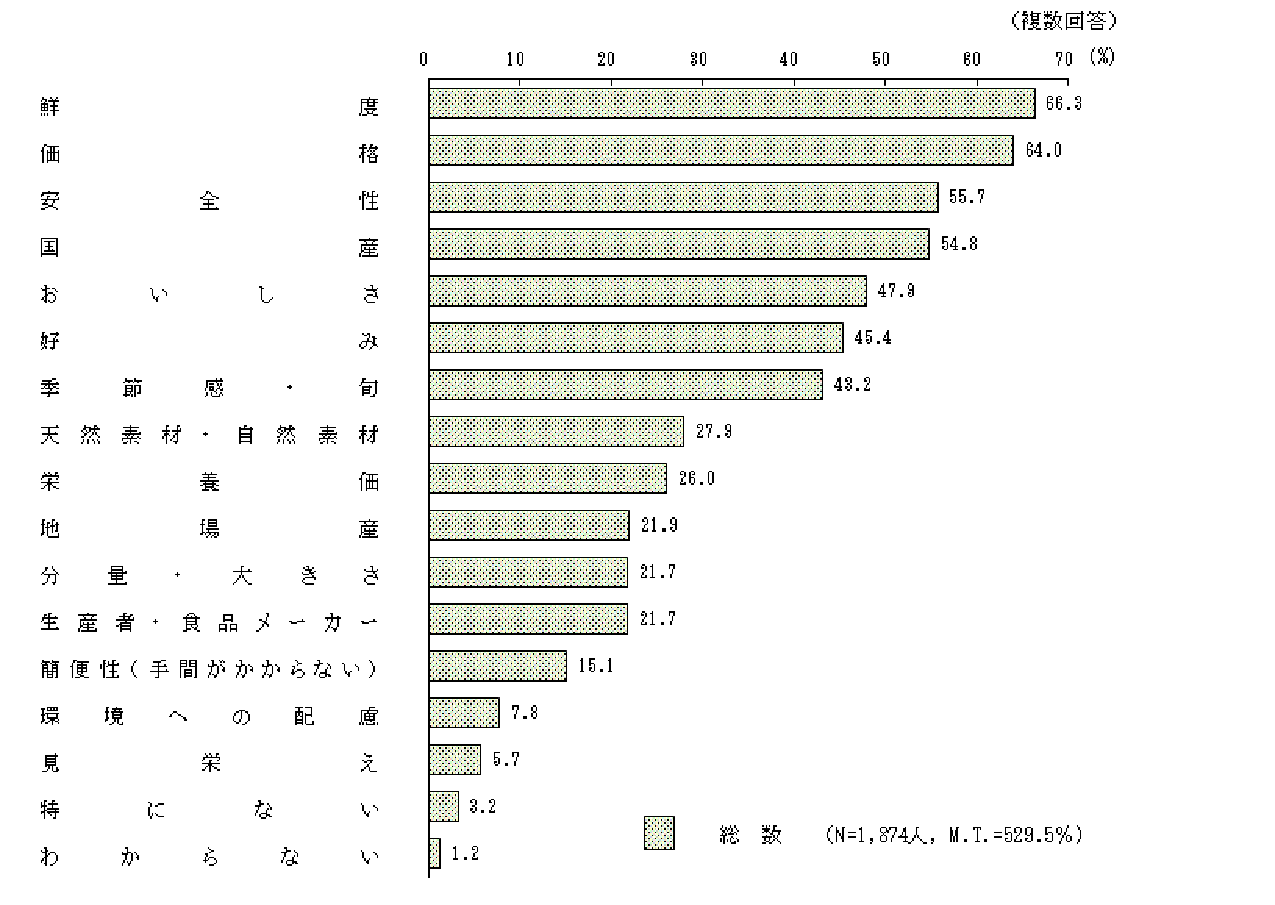
\includegraphics[width=1.0\linewidth]{Haraguchi_fig/syouhisyaanke-to.pdf}
	\caption{食品を選択する際に重視すること\protect\footnotemark[1]}
	\label{fig:zyuusi}
\end{figure*}
また,牛海綿状脳症(以下,BSE問題とする)や,食品偽装問題によって,食品の安全性や生産方法に関する消費者の意識は年々高まっている.
それに対応するように,日本国内では生産手法に関する取り決めとして,日本農林規格(JAS)や,米トレーサビリティ法など食品の安全性に寄与する規格やガイドラインが確立されてきた.しかし,消費者がこの認証規格の基準を知ることは困難である.また,有機農産物の認証情報の改ざんが問題視されている.さらに,生産者が認証を受けるまでにかかる管理コスト,認証にかかる費用などが高い.農林水産省有機JAS認定手数料\footnote{有機JAS認定手数料:\url{https://www.maff.go.jp/j/jas/jas_kikaku/pdf/yuuki_tesuryo_04.pdf}}によると個人農家が有機農作物の認証を受けるために,申請書年度に10万円,さらに年ごとに更新が必要であり,その更新費用は7万円である.生産者にとってはこのような高いコストを払ってまでの費用対効果があるのかが疑問である.このような中で,農産物認証をより信頼を持った形で消費者に伝えられるような仕組み,生産者が認証制度に加盟するためのインセンティブの設計が求められている.

本研究では,消費者がより信頼性を持った形で有機農産物の認証を確認でき,生産者が認証の加盟に対してよりインセンティブが働くために,有機農産物の認証を分散台帳技術を用いて実現し,消費者における信頼性の向上と,トレーサビリティの評価を行う.また,生産者にとってその認証方法が生産者にとって認証を取得するためのインセンティブになるのかを考察する.第2章では既存の農作物トレーサビリティと,認証モデル,その課題についての説明をする.第3章では分散台帳を用いたデジタル認証についての仕組みを説明する.第4章では,有機農産物の分散台帳による認証を有機キウイを取り扱った事例をケーススタディとしておこない,そのケーススタディを考察する.そして,第5章では妥当性への脅威の評価を行う.


\chapter{有機農産物の認証とトレーサビリティ}
\section{有機農産物認証の仕組み}
農産物の認証制度は日本の法律やガイドライン,都道府県や農業共同組合等の基準により化学肥料および化学農薬の低減や土づくりによる農産物の生産方式に対して農家や農産物を認証する制度であり,日本においては1950年に農林物資規格法として制定された.この法律の目的は適正な規格の制定・普及によって,農林物資の品質の向上,生産の合理化,取引の単純・公正化及び使用又は消費の合理化を図り,あわせて公共の福祉の増進に寄与することを目的としている\footnote{農林物資規格法:\url{https://www.maff.go.jp/j/jas/kaigi/attach/pdf/210104_7-1.pdf}}.この農林物資規格法は粗悪品の排除・ 食品・農林水産品の品質向上など,「農林水産物」そのものを対象としていた.この法律に基づいてできた認証制度がJapanese Agricultural Standards(JAS)である.さらに,1993年には品位,成分,性能の基準に加え,生産の方法についても基準の制定が可能となり,2017年の改正では題名を「日本農林規格等に関する法律」に改称し,規格の対象を,「生産方法」(プロセス),「取扱方法」(サービス等),「試験方法」などに拡大した.農業の生産方法に対して,環境への配慮や,持続可能性が重要視されるようになり,生産方法や管理などに反映されてきた,それに伴い,環境へ配慮した生産方法のガイドライン等が決められた規格が制定されていった.消費者はその規格に準拠されているのかを重要視し,商品を選択する.このように,環境保全や循環型社会,食の安全,安心などに関心が高まる中,化学肥料や農薬を使用しない,「有機農業」が注目を浴びるようになってきた.しかし,当時は有機農業のルールが制定されてなかったこともあり,1990年後半から有機農業に関する議論が行われ1999年に有機農産物の認証規格(有機JAS制度)が制定された.有機JAS制度は(Food and Agriculture Organization of the United Nations)とWHO(World Health Organization) によって設置された食品の国際規格を設定する機関であるコーデックス委員会~\footnote{codexalimentarius:\url{FAOhttps://www.fao.org/fao-who-codexalimentarius/world-food-safety-day/wfsd-homepage/en/}}(Codex Alimentarius Commission)の有機ガイドラインに準拠している.有機栽培における規格は,有機農産物の生産場所,有機農産物加工品の製造工場,など有機農産物の生産,製造,加工場所に対して認定を受ける.生産場所に対する有機農産物の生産の方法に関しては次のように明示されている.

\begin{enumerate}
    \item 農業の自然循環機能の維持増進を図るため,化学的に合成された肥料及び農薬の使用を避けることを基本として,土壌の性質に由来する農地の生産力(きのこ類の生産にあっては農林産物に由来する生産力,スプラウト類の生産にあっては種子に由来する生産力を含む.)を発揮させるとともに,農業生産に由来する環境への負荷をできる限り低減した栽培管理方法を採用したほ場において生産すること.
    \item 採取場(自生している農産物を採取する場所をいう)において,採取場の生態系の維持に支障を生じない方法により採取すること.
\end{enumerate}

このように,環境に配慮された生産方法を元にして,使用禁止農薬,栽培圃場への周辺からの使用禁止資材が飛来しないことなどの条件が明記されている.

図\ref{fig:yuukisikumi}は有機農作物の仕組みを示す.図\ref{fig:yuukisikumi}に示すように有機農産物の生産者はガイドラインに則って生産工程管理記録を記録し,有機農産物の登録認証機関に申請を行う.その後,登録認証機関が調査を行い,ガイドラインに準拠した生産工程が管理されていると判断された時登録認証機関が農林水産大臣へと申請を行い,有機農産物の認証を農林水産大臣が登録を行い,登録認証機関から生産者に対して認証が付与される.

有機農産物の認証が与えられた後は,生産者の出荷する農作物に図\ref{fig:JAS}\footnote{有機色食品の検査認証制度:\url{https://www.maff.go.jp/j/jas/jas_kikaku/yuuki.html}}で示すような有機JASマークを付与することができる.消費者は,この認証マークを確認することによって有機農産物の認証を受けた農産物であることを確認する.

有機農産物認証が付与されたのち,生産者は生産工程管理記録,格付管理記録,出荷管理記録に随時情報を記録する必要がある.生産工程管理記録は,農産物の種まきから収穫までの農薬や肥料の使用履歴等を記載する.また,格付け管理記録は収穫後の農産物の品質分類や格付け情報を記録する.出荷管理記録では農産物がどのように,いつ,どこへ出荷されたのかの詳細が記載される.特に,有機JAS認証マークの数を正確に把握するために,認証マークを幾つ付与したかなど正確に記入する必要がある.

これらの記録は有機栽培認証協会が,一年に一度監査に入り,圃場監査とともに検査を受ける.この際,有機農産物認証のガイドライン\footnote{有機食品の検査認証制度について:\url{https://www.maff.go.jp/j/jas/jas_kikaku/attach/pdf/yuuki-403.pdf}}に対する違反があれば,生産者に対して是正勧告を行う.もし,この是正勧告に従わなかった場合,または違反内容が悪質だった場合は生産者に対して出荷停止を命令することができる.このように有機栽培認証協会が定期的に監査を行うことで有機農産物の不正が行われないための抑止力となっている.

\begin{figure*}[t]
        \centering
	
\includegraphics[width=0.7\linewidth]{Haraguchi_fig/JASmark.pdf}
	\caption{有機JASマーク\protect\footnotemark[3]}
	\label{fig:JAS}
\end{figure*}

\begin{figure*}[t]
	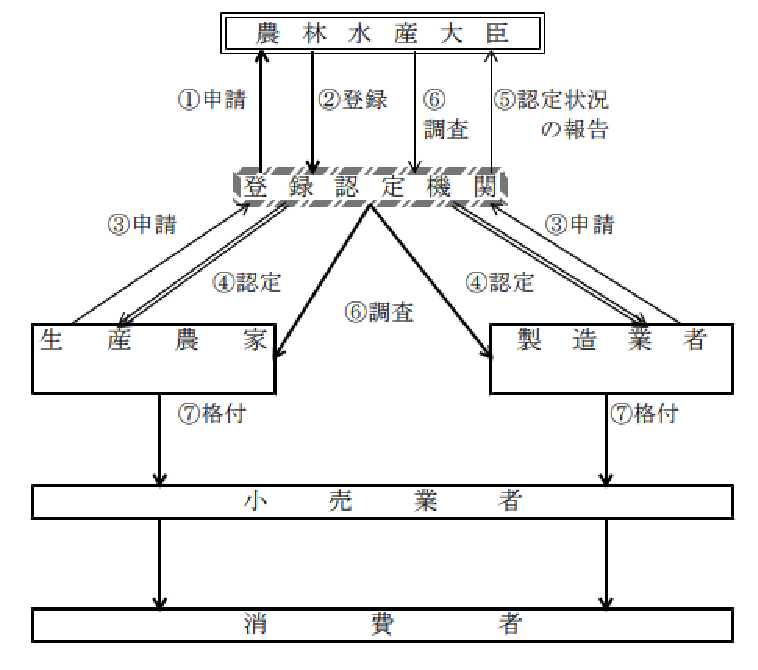
\includegraphics[width=1.0\linewidth]{Haraguchi_fig/yuukijaszentai.pdf}
	\caption{有機農産物の認証の仕組み\protect\footnotemark[4]}
	\label{fig:yuukisikumi}
\end{figure*}


\section{農産物トレーサビリティ}
トレーサビリティとは,商品の生産・流通過程が追跡可能であること,および,生産・流通の履歴を正確に記録・管理することである.特に食品におけるトレーサビリティは2004年コーデックス委員会」~\footnote{codexalimentarius:\url{FAOhttps://www.fao.org/fao-who-codexalimentarius/world-food-safety-day/wfsd-homepage/en/}}(Codex Alimentarius Commission)によって「生産,加工及び流通の特定の一つ又は複数の段階 を通じて,食品の移動を把握できること」と定義された.農産物におけるトレーサビリティは食品安全性の確保や品質管理を強化し,万が一の食品事故が発生した際に迅速な原因究明と対応を可能にする.トレーサビリティは商品情報が誰に届くのかを追跡することができるところと,その商品がどのような経路を経て消費者に届いたのかの訴求ができるところが特徴である.図\ref{fig:toresa}にあるように,商品にたいして問題が発生した際に追跡を行うことにより商品を回収でき,商品をたどった経路を訴求することで問題が発生した原因を明らかにすることができる.これにより,消費者の信頼を高め,より安心して農産物を購入できるようになる.トレーサビリティはこれまでは製造業で中心に言われていたことであるが,2000年に発生した牛肉のBSE問題や産地偽装問題によって,食品業界全体に対してもトレーサビリティの重要性が増してきた.日本では,BSE問題をきっかけとして農林水産省が2003年に「牛の個体識別のための情報の管理及び伝達に関する特別措置法(牛トレーサビリティ法)」を制定した.この法律では,牛への耳標の装着,出生から牛肉になるまでの履歴情報の届出・記録・保存,記録された情報のインターネットでの公表などが定められている.また,2008年に起きた事故米(汚染米)不正転売事件の反省から,農林水産省は翌年2009年に「米穀等の取引等に係る情報の記録及び産地情報の伝達に関する法律」(米トレーサビリティ法)を制定している.こちらは米の生産農家が流通業者小売業者と取引をする際に7つの項目を記載することが必要とされている.

1.品名

2.産地

3.数量

4.年月日

5.取引先名

6.半出入した場所

7.用途を限定する場合にはその用途等

これらは,実際の取引において取り交わされる伝票または帳簿にて記録されるようになっている.

\begin{figure*}[t]
	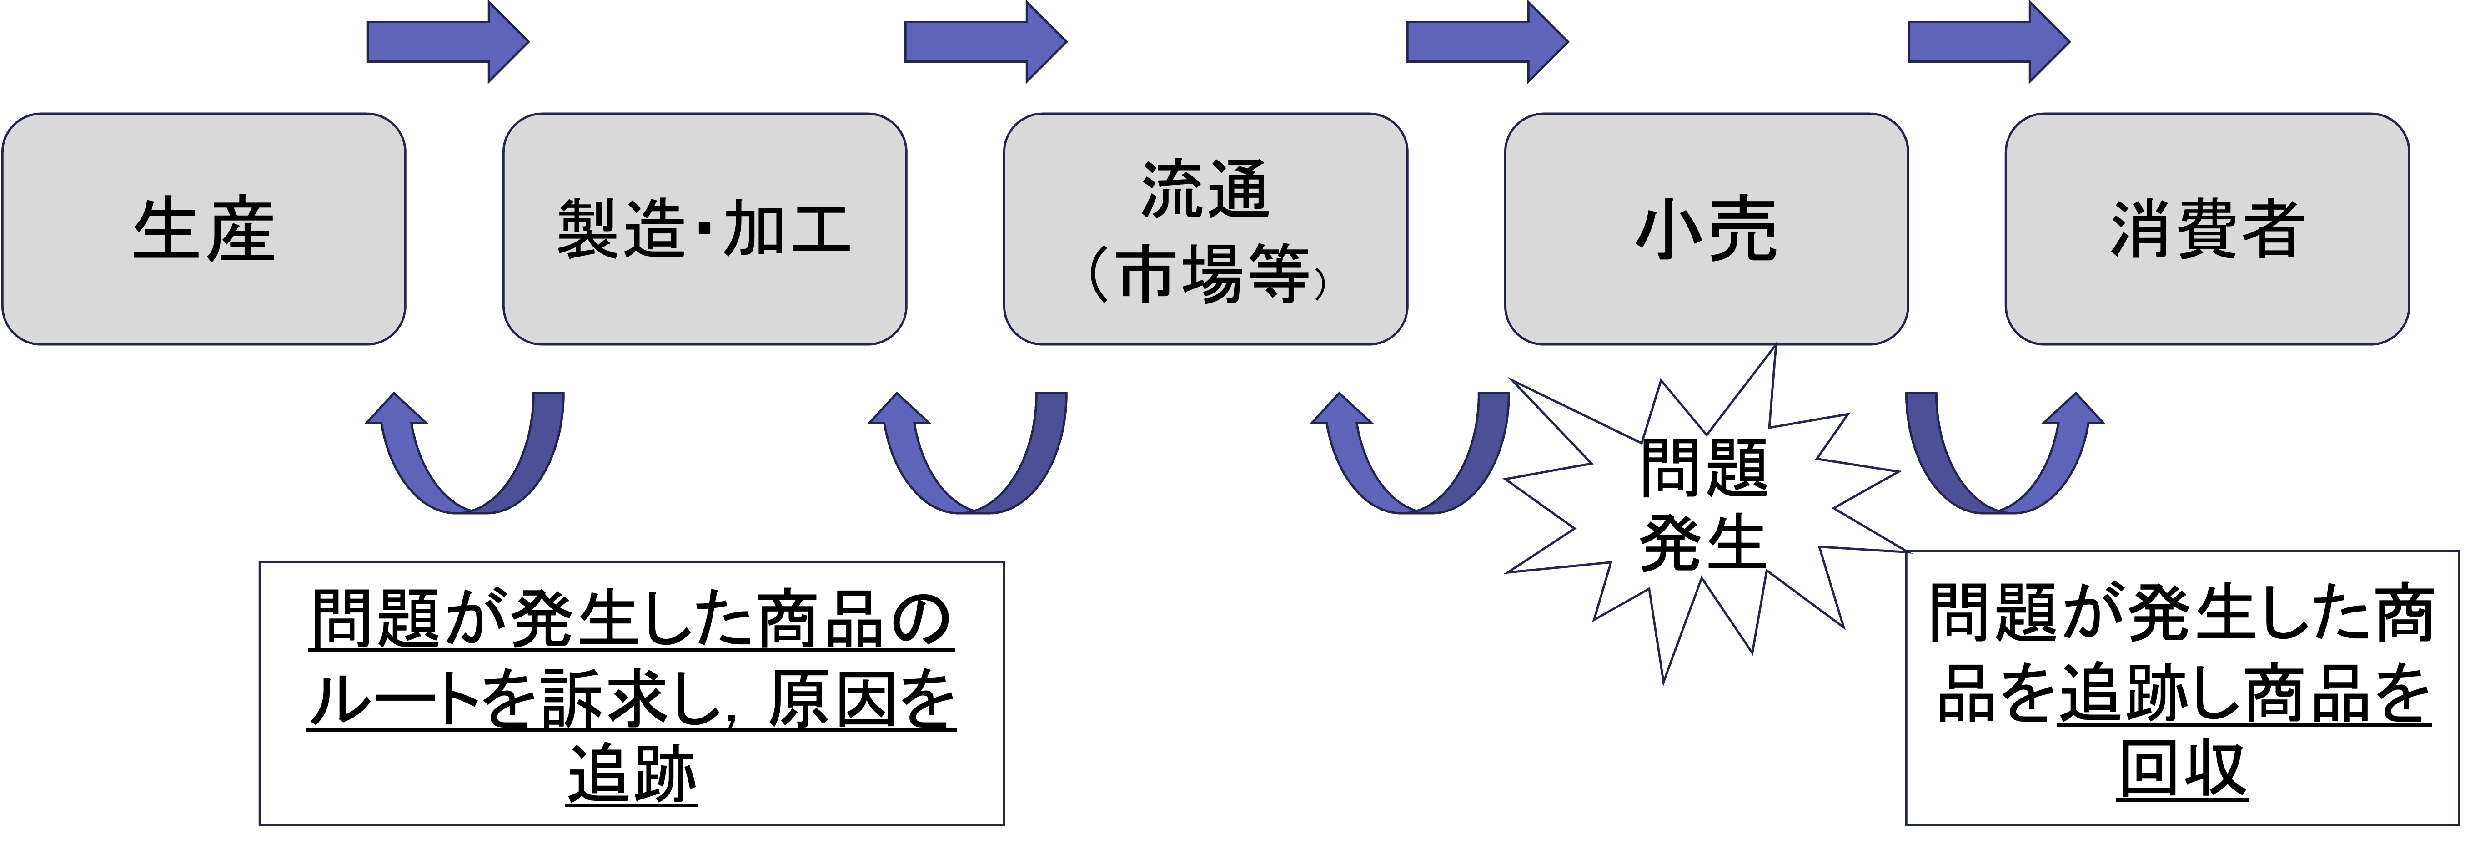
\includegraphics[width=1.0\linewidth]{Haraguchi_fig/toresa.pdf}
	\caption{食品のトレーサビリティ}
	\label{fig:toresa}
\end{figure*}

\section{従来の認証における課題}
有機農産物における認証は,消費者にとって信頼性が十分であるとは言い難い.吉松らは現状の有機農産物における認証では食品偽装が混入する可能性は否定できないと指摘している\cite{2009}.また,消費者が有機農産物の商品を選択する際において,判断基準となるのが有機JASの認証マークだけであり,その他の栽培方法,生産地情報に関しては消費者が確認することは困難である.特にトレーサビリティの重要性は先に述べた通りだが,この有機農産物の認証マークではトレーサビリティをとることは容易ではない.有機農産物の認証においては,事業者内では記録を残すことが必要となっているが,現在の認証方法では有機農産物認証を取得するために,事業者間での情報は共有されない.これでは,有機農産物の流通全体でのトレーサビリティを確保するために情報を共有することが困難であるとの指摘がある\cite{yuuki}.一方,農業生産者にとって有機農産物の認証においては第三者認証機関である有機農業認証協会が,生産者の提出する生産工程管理記録を確認したのち実地検証等によって生産場所に対して認定する.しかし,認定を受けるためには有機農産物のガイドラインに則った栽培方法を2年以上続け,栽培の管理方法を記録する必要があり,その管理記録も膨大な量となる.また,有機農作物の認証を受けるためにかかる費用が10万円,年ごとの更新費用も7万円かかり,生産者にとっては大きな負担となる.松岡らはこの管理にかかる労働コストと金銭的なコストは有機農産物の価格に転嫁されるが消費者にとって有機農産物というだけでこの価格に耐えうる消費者は多くないと指摘している\cite{matsuoka}.本研究では,有機農産物の認証をトレーサビリティを担保し,生産者が高いコストを払ってでも有機農産物の認証を取得できる手法を提案し,ケーススタディによって考察する.

\begin{figure*}[t]
	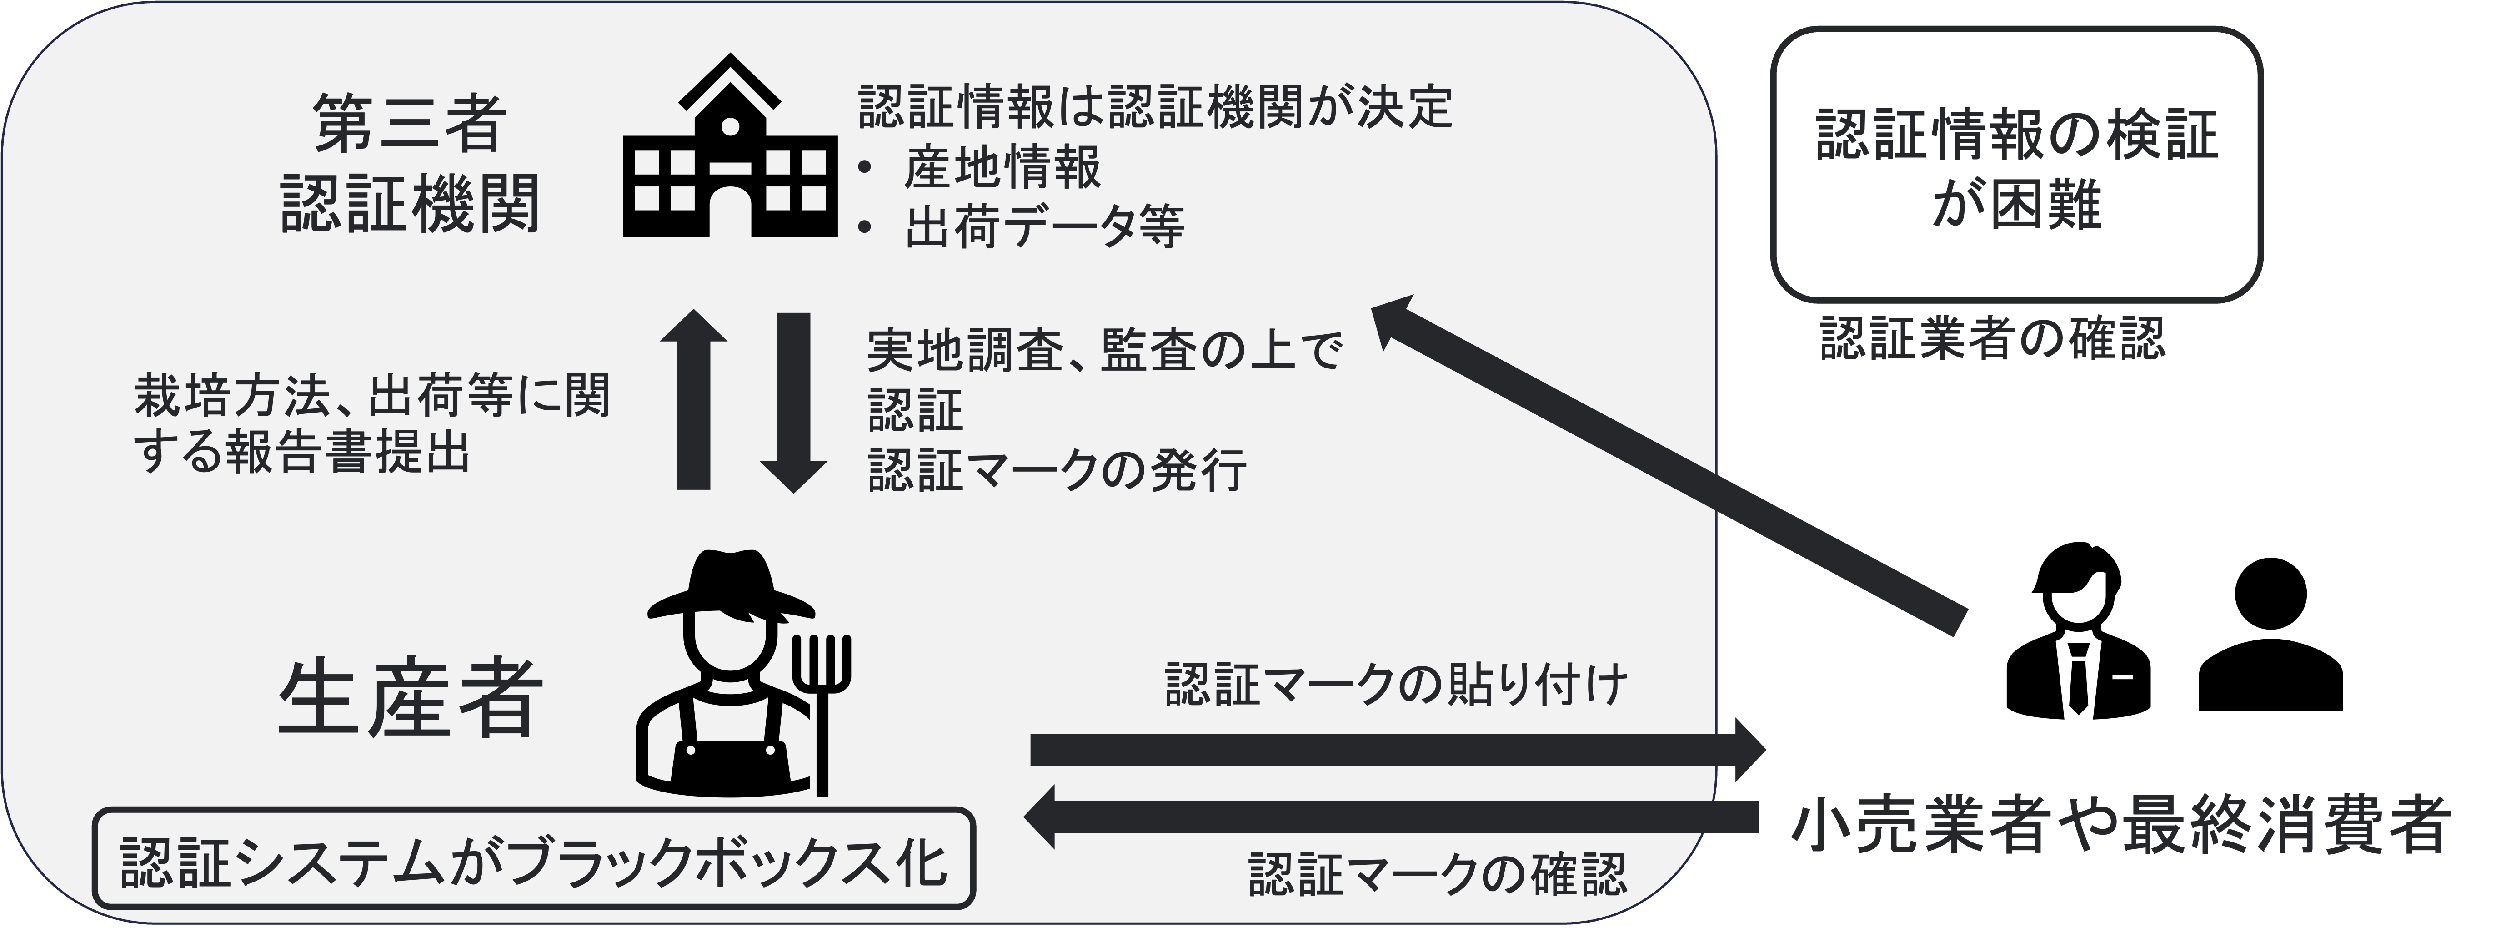
\includegraphics[width=1.0\linewidth]{Haraguchi_fig/blackbox.pdf}
	\caption{認証における課題}
	\label{fig:blackbox}
\end{figure*}

\chapter{農産物のデジタル認証}

この章では,有機農産物をトレーサビリティを担保した形で,認証を取得するために使用する分散台帳技術とそれに関連する技術に関して説明する.また,その技術による関連研究を示し,その関連研究での概要と課題に関して説明する.

\section{分散型台帳技術,DID}
分散台帳技術(Distributed Ledger Technology:DLT)とは,複数のコンピュータが同じデータを共有,管理しており,ネットワーク参加者全員で台帳を管理することができる技術である.図\ref{fig:bunnsan}のように一般的な情報システム,データベースでは台帳情報が一元管理され,中央管理者がいることが一般的であるが,分散台帳技術ではその管理者が存在せず,中央集権型のサーバーも存在しない.分散台帳は各コンユーターがピアツーピア(P2P)ネットワークによってつながっており,分散化,透明性を確保するためにブロックチェーン上に保存され,実行される.また,情報を伝達する際には,何らかのインプットに対して,インプットの文字列の長さに関わらず,固定の長さのアウトプットを出力するハッシュ値によりデータを圧縮する関数が用いられる.この情報を公開鍵暗号技術と呼ばれる暗号化と複合をするための鍵が異なってペアになっている暗号化方式が用いられている.また,この鍵は本人のみが用いる秘密鍵と誰でも利用可能な公開鍵の2つに分けることにより,情報の選択的情報開示を可能としている.これらの技術によって,実質的に情報の改ざんが不可能な形で台帳上を共有することが可能となる.また,これらの開発はスマートコントラクト(SC)を書くことによって開発される.

この,分散台帳技術による認証をする際に,特に重要となる技術が,DID(Decentralized Identifier)である.DIDは,分散型台帳技術(DLT)を活用した新しい形式の識別子であり,個人や組織がオンラインで自己主権を持ち,自身のアイデンティティを管理できるように設計されている.このシステムは,中央集権型の認証機関に依存せずに,アイデンティティの検証と管理を行うことができる点が特徴である.DIDは図\ref{fig:did}のように「did:example:123456789haraguchitaku」といった一意の識別子で表され,これによりDID所有者はインターネット上で一意に識別される.DIDはDIDドキュメントにリンクされており,このドキュメントは公開鍵,認証方法,サービスエンドポイントなど,DID所有者に関する情報を含んでいる.DIDドキュメントはブロックチェーンやその他の形式のDLT上に保存され,データの不変性と公開アクセスが保証される.DIDの仕組みは,DID所有者が自身のアイデンティティ情報を完全にコントロールできるようにすることで,プライバシー保護とセキュリティを強化する.たとえば,DIDを使用することで,ユーザーはオンラインサービスにログインする際にDIDを提供し,DIDドキュメント内の公開鍵を用いて認証プロセスを行うことができる.このプロセスにより,パスワードなどの従来の認証手段に比べて,セキュリティが向上する.さらに,DIDシステムは選択的情報開示を可能にする.これは,ユーザーが自分に関する情報を共有する際に,必要最小限の情報のみを選択的に開示できる機能である.例えば,年齢確認が必要なサービスを利用する場合,ユーザーは自分の具体的な生年月日ではなく,「法定年齢以上である」という事実のみを証明することができる.これにより,プライバシーの保護が強化される.

\begin{figure}[t]
  \centering
  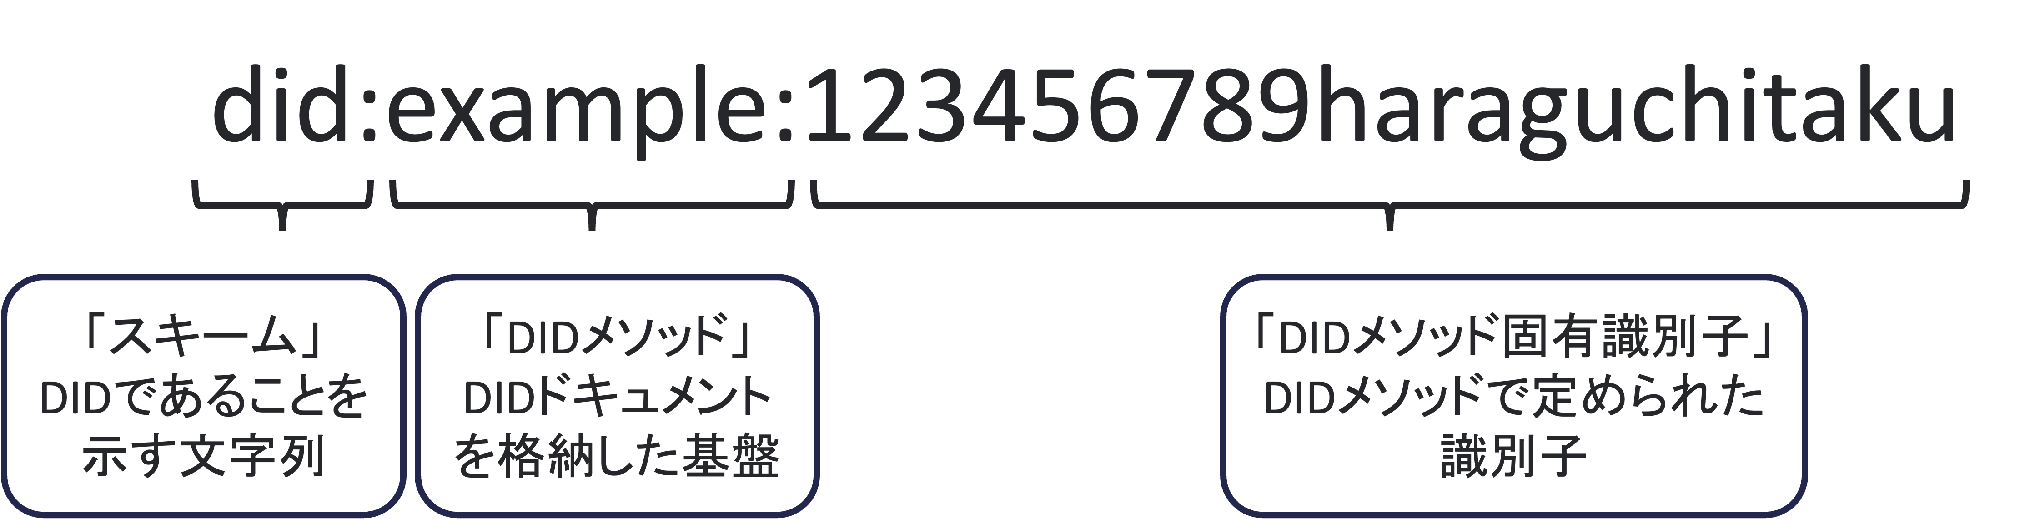
\includegraphics[width=1.0\linewidth]{Haraguchi_fig/DID.pdf}
  \caption{DIDの構造}
  \label{fig:did}
\end{figure}

DIDシステムの実装には,ブロックチェーン技術が中心的な役割を果たす.ブロックチェーン上にDIDドキュメントを保存することで,データの透明性と不変性を保証し,DID所有者と第三者との間で信頼を構築する.また,DIDはデジタル署名や暗号化通信にも使用され,オンライン取引の安全性を高める.DIDは,オンラインでのアイデンティティ管理において革新的なアプローチを提供し,ユーザーが自身のデジタルアイデンティティをより安全に,かつ自由に管理できるようにする.この技術は,プライバシーの保護,セキュリティの向上,ユーザー主導のアイデンティティ管理の促進に寄与すると期待されている.

\begin{figure}[t]
  \centering
  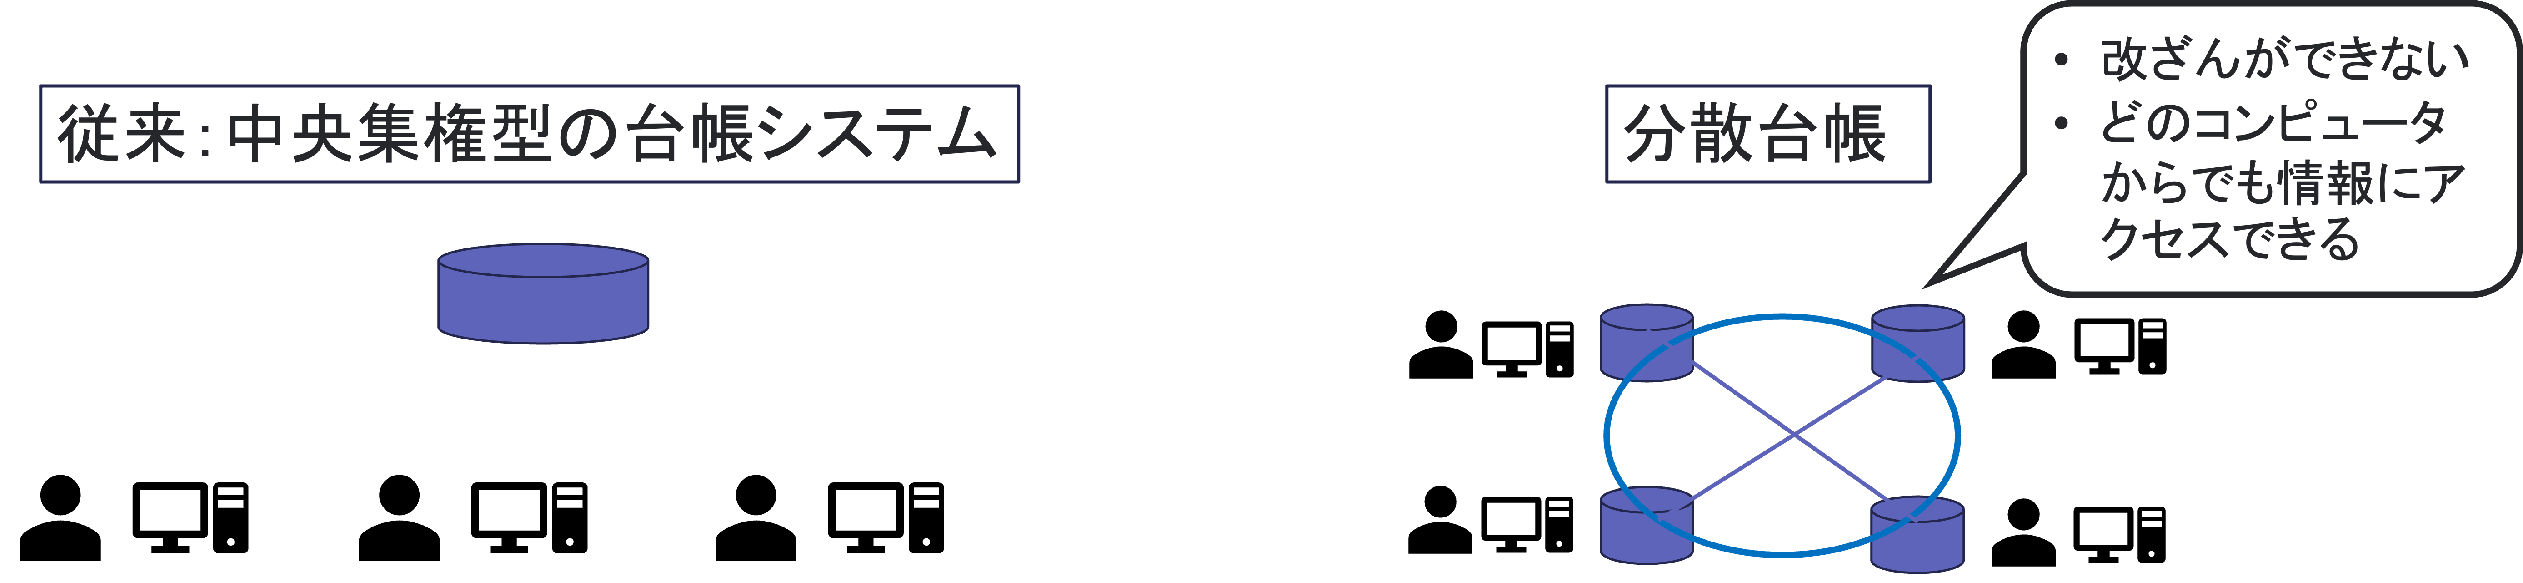
\includegraphics[width=1.0\linewidth]{Haraguchi_fig/bunnsan.pdf}
  \caption{既存システムと分散台帳}
  \label{fig:bunnsan}
\end{figure}


\section{分散台帳によるデジタル証明}

ブロックチェーン技術を用いたデジタル認証は,分散型台帳技術(DLT)を基盤として,取引の透明性,不変性,およびセキュリティを実現する手法である.デジタルアイデンティティ,契約,証明書などの認証情報をブロックチェーン上に記録し,その情報の検証を可能にすることで,第三者の介入なしに信頼性の高いデジタル認証を提供する.図\ref{fig:did}では,そのデジタル認証がどのように行われているのかの概要を示している.デジタル認証のプロセスは,分散型識別子(DID)と検証可能な資格情報(VC)に基づいている.DIDは,ユーザーが自分のデジタルアイデンティティを管理し,異なるサービスや組織と安全に相互作用するための分散型手段を提供する.VCは,ユーザーが自分のアイデンティティに関する信頼できる情報を第三者に提供し,検証するためのデジタル形式を提供する.これらの資格情報は,日常生活で使用される身分証明書や運転免許証などのデジタル等価物として機能し,選択的開示をサポートして,ユーザーが必要な情報のみを提供することが可能となる.ここでの選択的情報開示(Selective Disclosure)とは,セルフ・ソブリン・アイデンティティ(SSI)に基づく認証メカニズムの重要な特徴の一つである.選択的情報開示により,ユーザーは自身のアイデンティティ情報を共有する際に,必要最低限の情報のみを提供することが可能となりこれは,プライバシーの保護とデータの最小化原則を実現するために不可欠である\cite{dezital}.具体的には,法定年齢以上であることの証明など,ユーザーがオンラインで特定のアクションを実行する必要がある場合,選択的情報開示をサポートする検証可能な資格情報を使用して,その主張を証明することができる.さらに,Luxらはゼロ知識証明(Zero-Knowledge Proof)を用いることで,年齢が法定年齢を超えていることを証明しながら,具体的な生年月日を開示することなく,プライバシーを保護することができると述べている\cite{dezital}.

\begin{figure*}[t]
	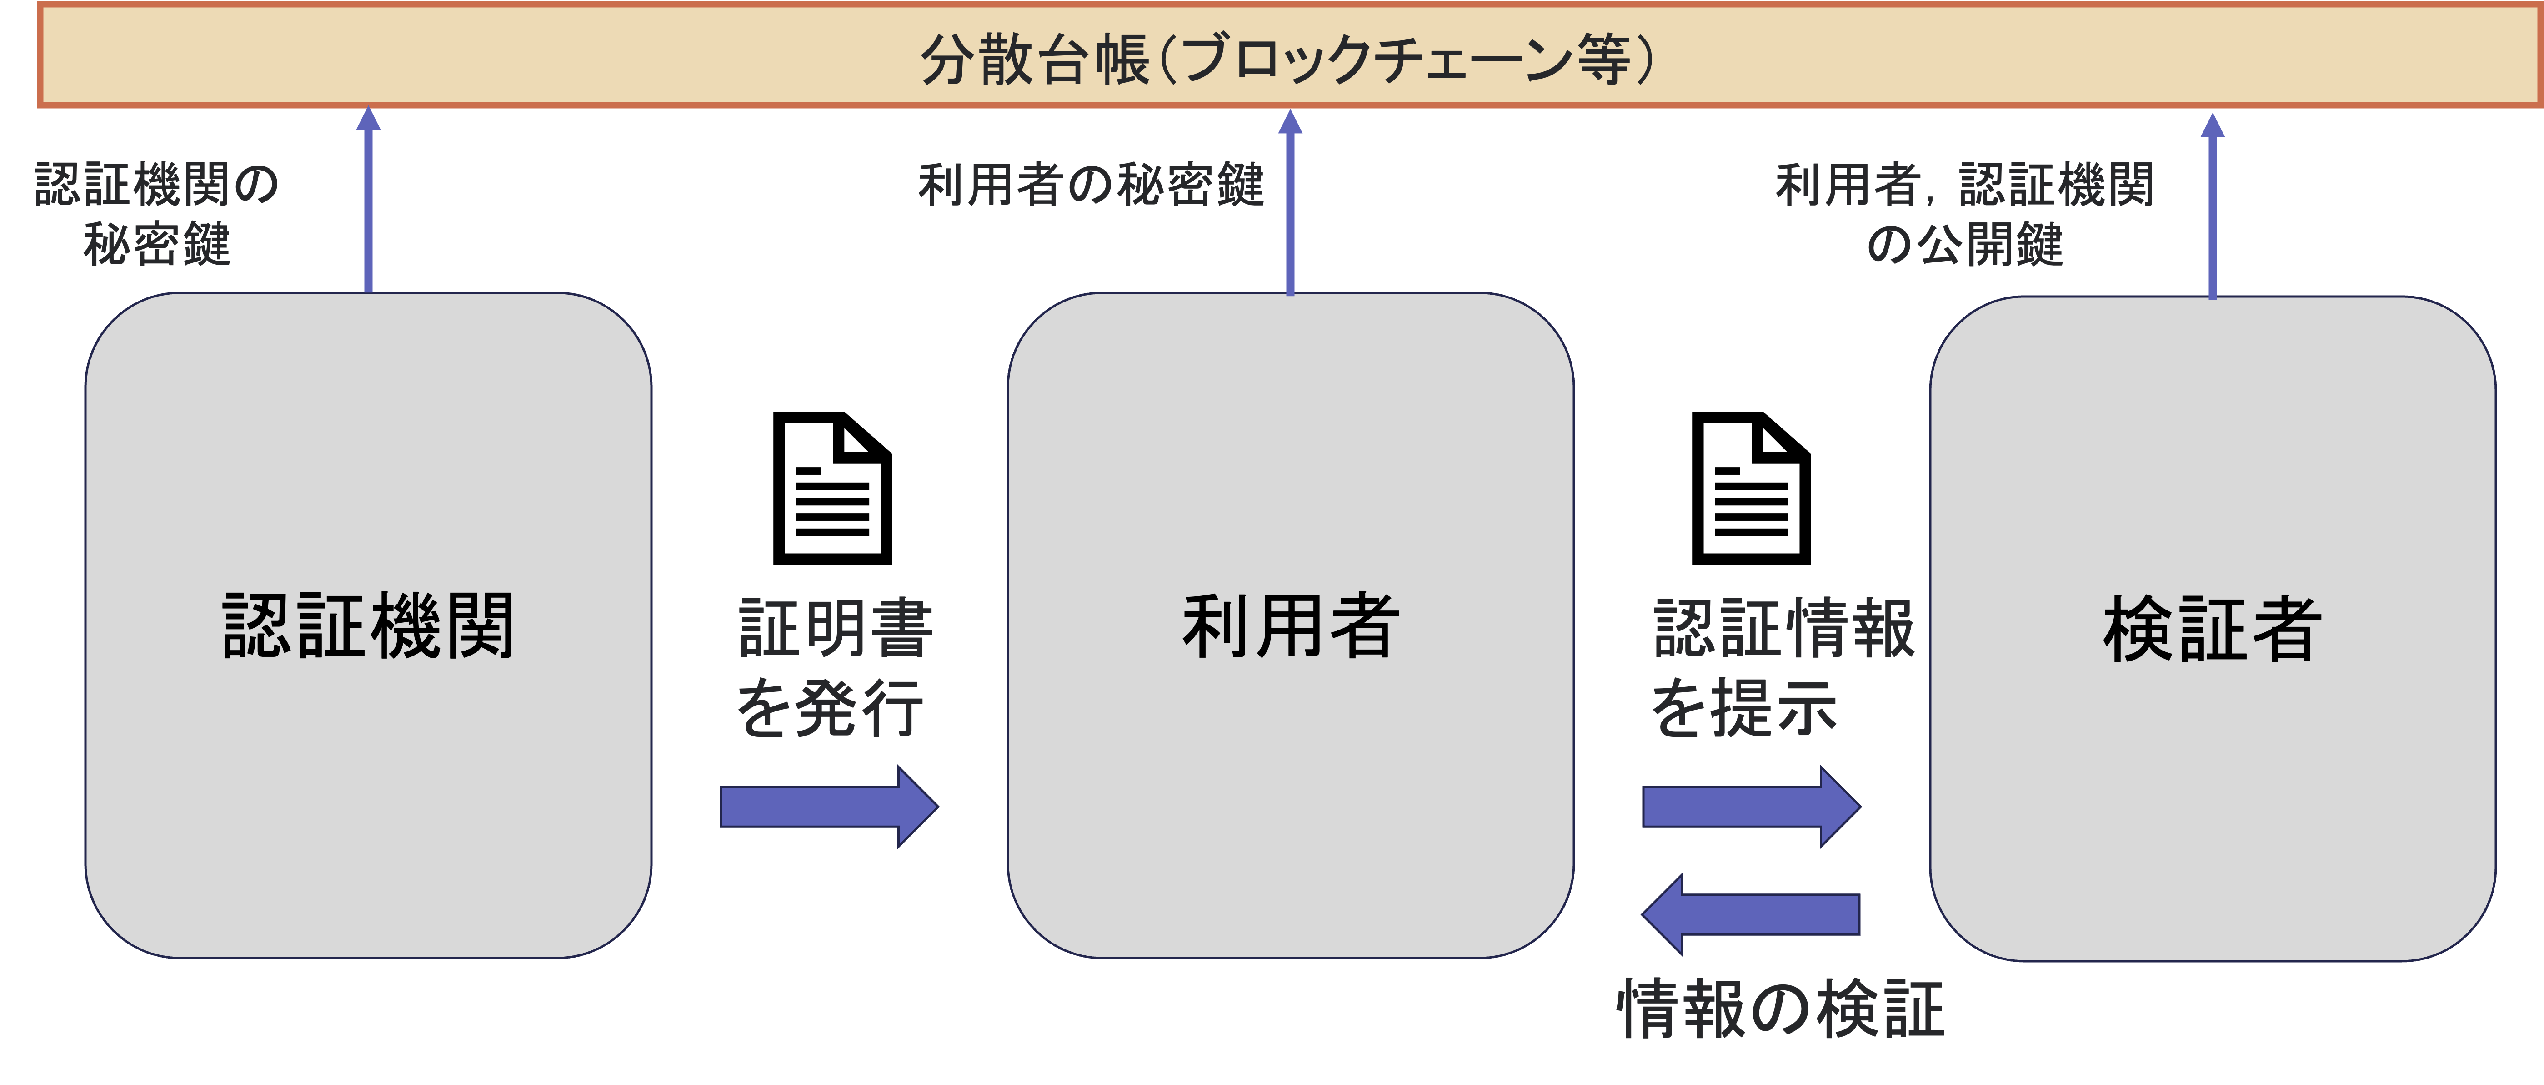
\includegraphics[width=1.0\linewidth]{Haraguchi_fig/dezitaruni.pdf}
	\caption{分散台帳を用いたデジタル認証の概要}
	\label{fig:ninteisyou}
\end{figure*}


\section{関連研究}
分散台帳技術の多産業への応用事例は様々なされているが,Geらは金融,産業,社会などさまざまな産業において分散台帳技術の応用について大きな関心ごとになっていると指摘している\cite{yuukisukunai}.

分散台帳技術はBitCoinを起源として発展してきたが,現在は仮想通貨以外にもさまざまユースケースが提案されている\cite{weko_197995_1}\cite{hearth}\cite{buturyu}.
分散台帳技術の期限であるビットコインでは,誰もがネットワークへと参加することが可能となっているが,法人間のビジネスにおけるユースケースではネットワークの参加者を制限する必要がある.河田らによると金融においては情報の改竄性の観点から金融取引において分散台帳技術の応用が期待されるが,信頼される取引が秘匿性を担保されるためにはいくつかの課題があることを指摘している\cite{hearth}.bourasらによると医療分野における分散台帳技術への可能性を示唆しており,分散台帳技術を用いたアイデンティティ管理システムの構築により,患者が自身のアイデンティティを完全にコントロールできるようになり,データの不変性における信頼が向上することが可能になると述べられている.
分散型アイデンティティ管理(IdM)の主要な要件であるガバナンス,パフォーマンス,アクセシビリティ,プライバシーを既に満たしており,分散型台帳技術を使用して,手続きやステークホルダー間でのヘルスケア情報の統合をサポートする可能性があると説明している.しかし,SSIモデルをヘルスケア領域に適用することには,データ標準化,アクセス許可レベル,スケーラビリティの制限,参加とインセンティブのための採用,IdMコンセンサスプロトコルなど,さまざまな課題が見受けられる.marcelらは物流およびサプライチェーン管理における分散型アプリケーションであるHIDALS(Hybrid IoT-based Decentralized Application for Logistics and Supply Chain Management)について述べており,分散型台帳技術とIoTデバイスを統合して,組織間での高価値貨物の輸送を追跡し,契約違反を検出するシステムを提案した\cite{buturyu}.このシステムは,分散台帳技術のピアツーピアのモデルを応用し,異なる物流会社間の信頼とトレーサビリティを高め,消費者に対してSLAの遵守に関する証明を提供することを可能としている.また,ブロックチェーンを使用して所有権とSLA違反を不変かつ分散型の方法で追跡し,IoTデバイスを含むセンサーを使用してSLA違反を監視および追跡する.

農産物における分散台帳を用いた認証制度やトレーサビリティにおける研究は分散台帳における全体の応用例としては数は少ないが,いくつかの先行研究がなされている.Sachinらによる研究では農産物の流通全体のサプライチェーンにおけるトレーサビリティを分散台帳技術を用いて,可視性を上げる研究がなされている\cite{nousa}.この研究では,まず,既存のトレーサビリティシステムのデータの不一致性,相互運用性の欠如,可視性が低く透明性が担保されていないところを課題として挙げており,トレーサビリティシステムに対する分散台帳技術の有効性を定量的に評価を行った.そして農業サプライチェーンにおける分散台帳技術の導入を促進するための要因を特定し,それらの間の因果関係を確立することを目的として挙げている.しかし,この手法では,システムとしての有効性は示唆されているが,実際に現場レベルでの実装となると,農産物の流通に関わる全てのステークホルダーのシステムの一新が必要となり,それにかかる導入コストや,導入するためのインセンティブの議論がなされていない.BINらによる研究ではモモジュース製造における品質管理システムを分散台帳を用いたシステムにおいて実装しており,品質管理を人の手を加えず全てスマートコントラクトで実装モデルを構築した\cite{zyusu}.本研究では,生産工程の最適化を回帰分析手法に基づいた応答曲面法(RSM)によって行い,品質管理モデルであるPCA法を用いて商品自体の品質評価を自動的に行いつつ,そのプロセスを分散台帳上で改ざんができない形で管理するというものである.

\section{キーアイデア}
消費者にとって農産物の認証に関してその商品が本当に認証を受けたものであるのか,また,その認証がどのような形で認証されたのかトレーサビリティを確保した形で確認できることが必要である.しかし,現在の農産物認証においてはそこの確認が容易ではない.また,生産者にとっても農産物認証を取得,継続するためには金銭的コスト,労働コストもかかるため,認証を取得することにおいてのインセンティブの設計が必要となる.そのためには消費者にとっても有機JAS認証の商品をより選択する仕組みづくりが必要である.
分散台帳における認証は他の業種では様々な形として応用されていおり,信頼性を向上させるための技術として注目を浴びている.本研究では有機農産物認証においてもより消費者が検証しやすい形でかつ,生産者にとっても認証を取得するためのインセンティブを与えることを実現する可能性がある.本研究ではこの分散台帳を用いた有機農産物認証を有機キウイを扱う生産業者をケーススタディとして用い,消費者はもちろん,著者は3年キウイの生産に関わっているため,生産者両者の視点で,先述した課題を解決可能かどうかの議論を行う.

\chapter{ケーススタディ:有機キウイを用いた分散台帳による有機栽培の認証}

\section{有機農産物の分散台帳を用いた認証の流れ}
 有機キウイを有機農産物認証を取得したのち,分散台帳上に乗せ,消費者に届くまでは次のステップが必要となる.
 
\begin{itemize}
  \item 有機キウイの生産工程管理記録を記録し,有機栽培認証協会に提出する.
  \item 有機認証協会が生産工程管理記録の確認,圃場実地調査を経て,有機農産物として圃場に対して認定する.
  \item 有機認証協会が分散台帳上に認定証を上げ,生産者に対してデジタル形式で付与する.
  \item 有機キウイに有機JASとQRコードを付与する.
  \item 有機キウイを小売業者に納品する.
  \item 消費者が有機キウイを購入し,QRコードから有機農産物の検証,その他の生産者の情報を確認する.
\end{itemize}

\begin{figure*}[t]
	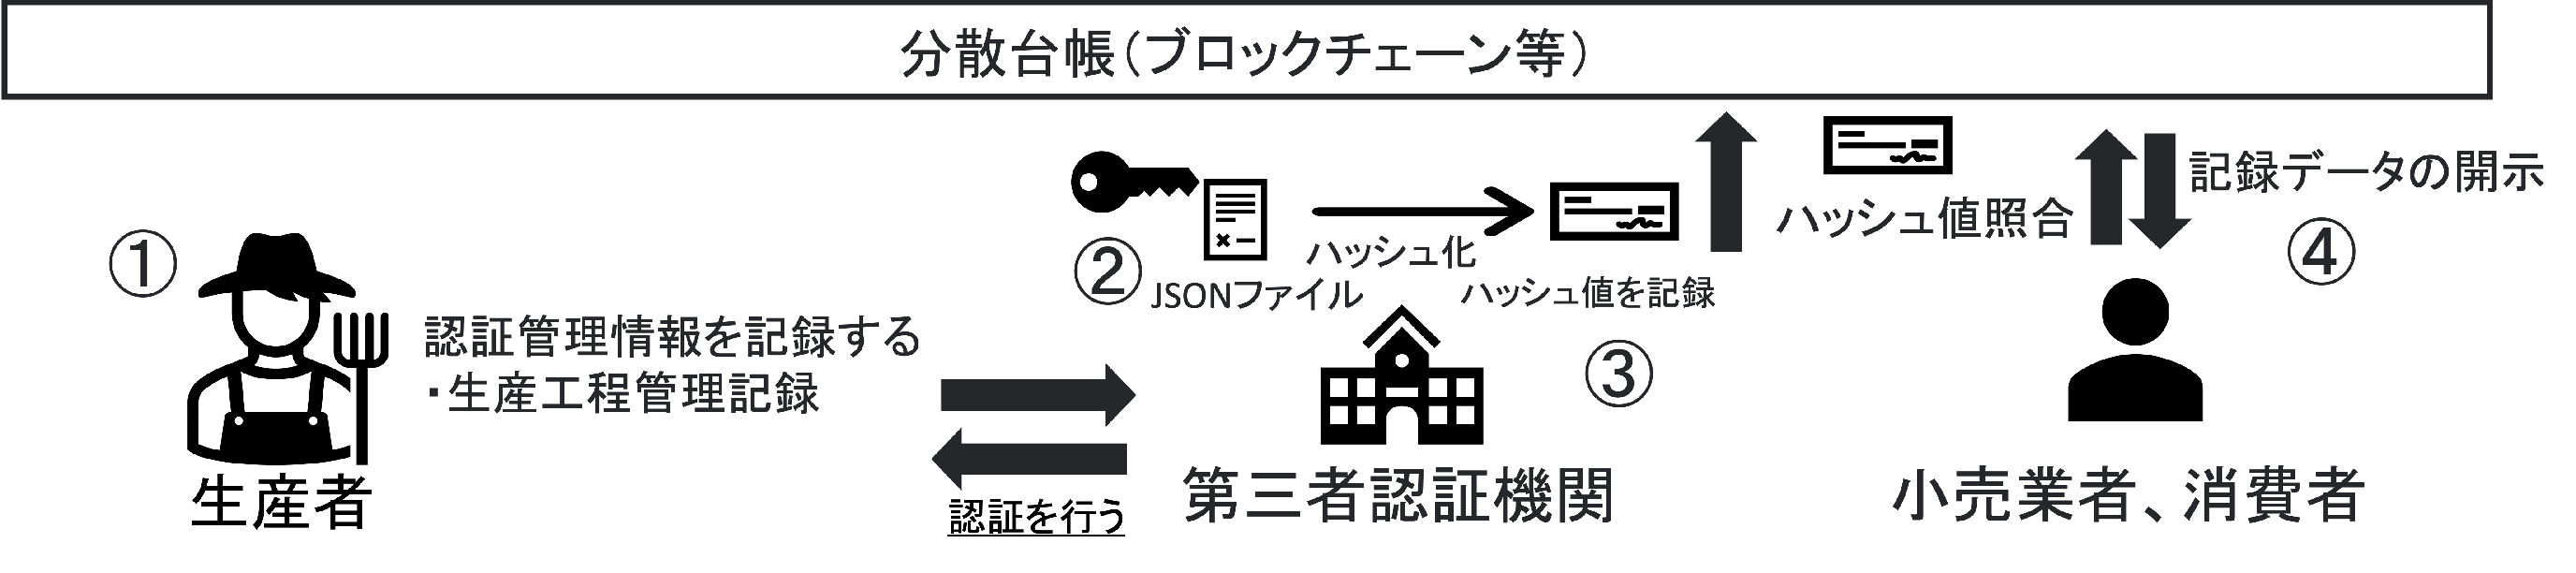
\includegraphics[width=1.0\linewidth]{Haraguchi_fig/shikumi.pdf}
	\caption{認証から消費者検証までの流れ}
	\label{fig:blackbox}
\end{figure*}


 
有機農産物の認証に関しては,有機栽培認証協会の講習会への参加,栽培の管理記録,実地圃場の調査,登録機関への申し込みと承認が必要である.ここで,栽培記録の管理記録に関しては有機栽培認証協会が出している生産工程管理記録を採用した.そして,その生産管理と圃場実地調査によって,認証された証明書をを分散台帳上に記録し,消費者に届くまでのケーススタディを行う.ケーススタディに用いるデータは株式会社ReFruitsのキウイの生産管理記録を元に擬似的に作成したものである.

図\ref{fig:Teiannsyuhou}はキウイの出荷を元にした生産工程管理記録の記録データである.こちらの記入したデータは第三者認証機関である有機栽培認証協会が審査を行い,圃場実地調査を経て有機農産物としての認証が降りるのかが判断される.この記録は,株式会社ReFruitsが生産するキウイの実際の生産管理記録をもとに擬似的に作成されたデータを使用している.


\begin{figure*}[t]
	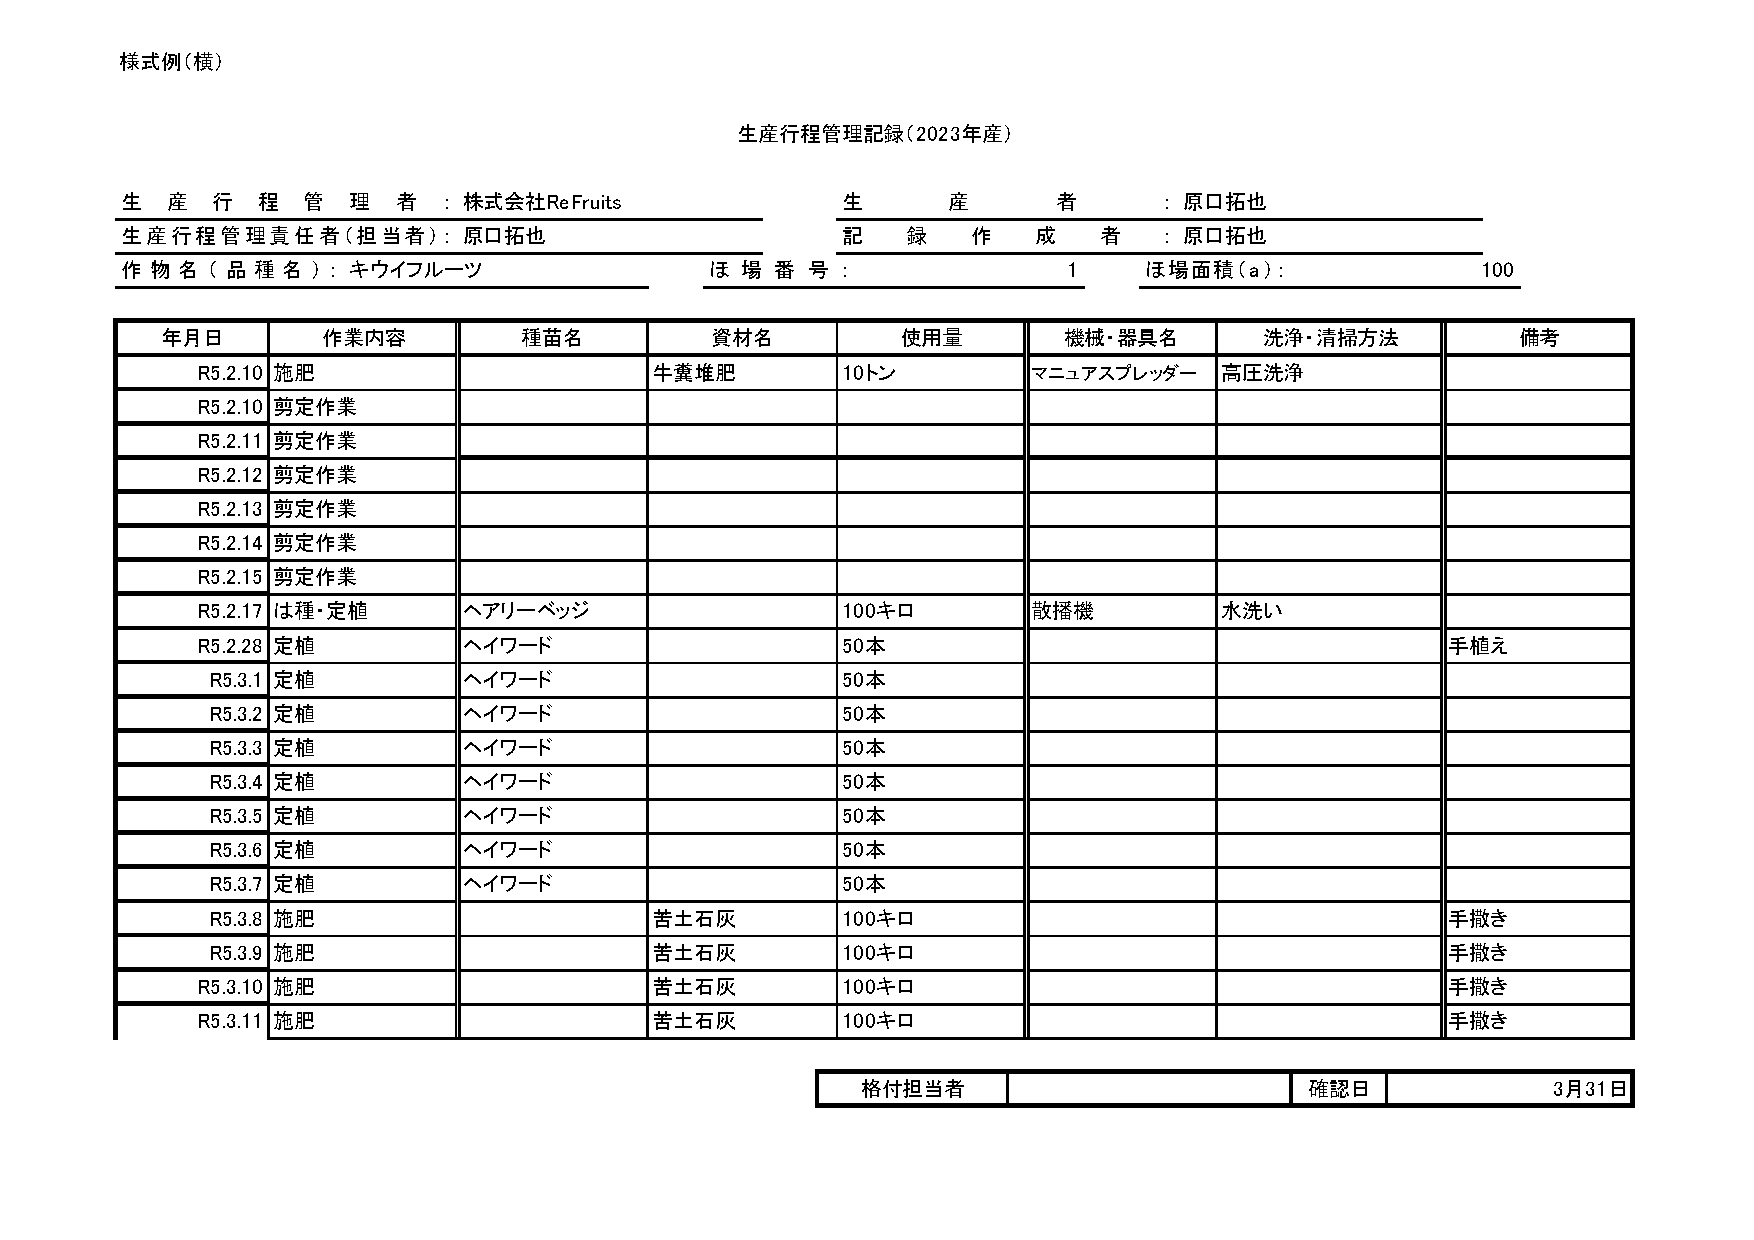
\includegraphics[width=1.0\linewidth]{Haraguchi_fig/seisannkoutei.pdf}
	\caption{生産工程管理記録}
	\label{fig:Teiannsyuhou}
\end{figure*}


\section{分散台帳による認証}
次に栽培管理記録を経て認証が降りる段階で,分散台帳上に認証を得た認定証を分散台帳上に記録する.この記録は,生産者が栽培管理記録を分散台帳技術を用いて記録することで,データの透明性,追跡可能性,不変性を確保する.分散台帳上に記録されたデータは,改ざんが困難であり,認証過程における信頼性を高める.図\ref{fig:ninteisyou}は有機農産物の認定証を示す.この認定証は,有機栽培認証協会が,認証を承認したのち,分散台帳上に認証情報を載せ,その認証データを生産者に付与する.この際用いる分散台帳のデータに関しては,BlockCertsの規格を元に,認定証を分散台帳上へアップロードする.

\begin{figure*}[t]
        \centering 
	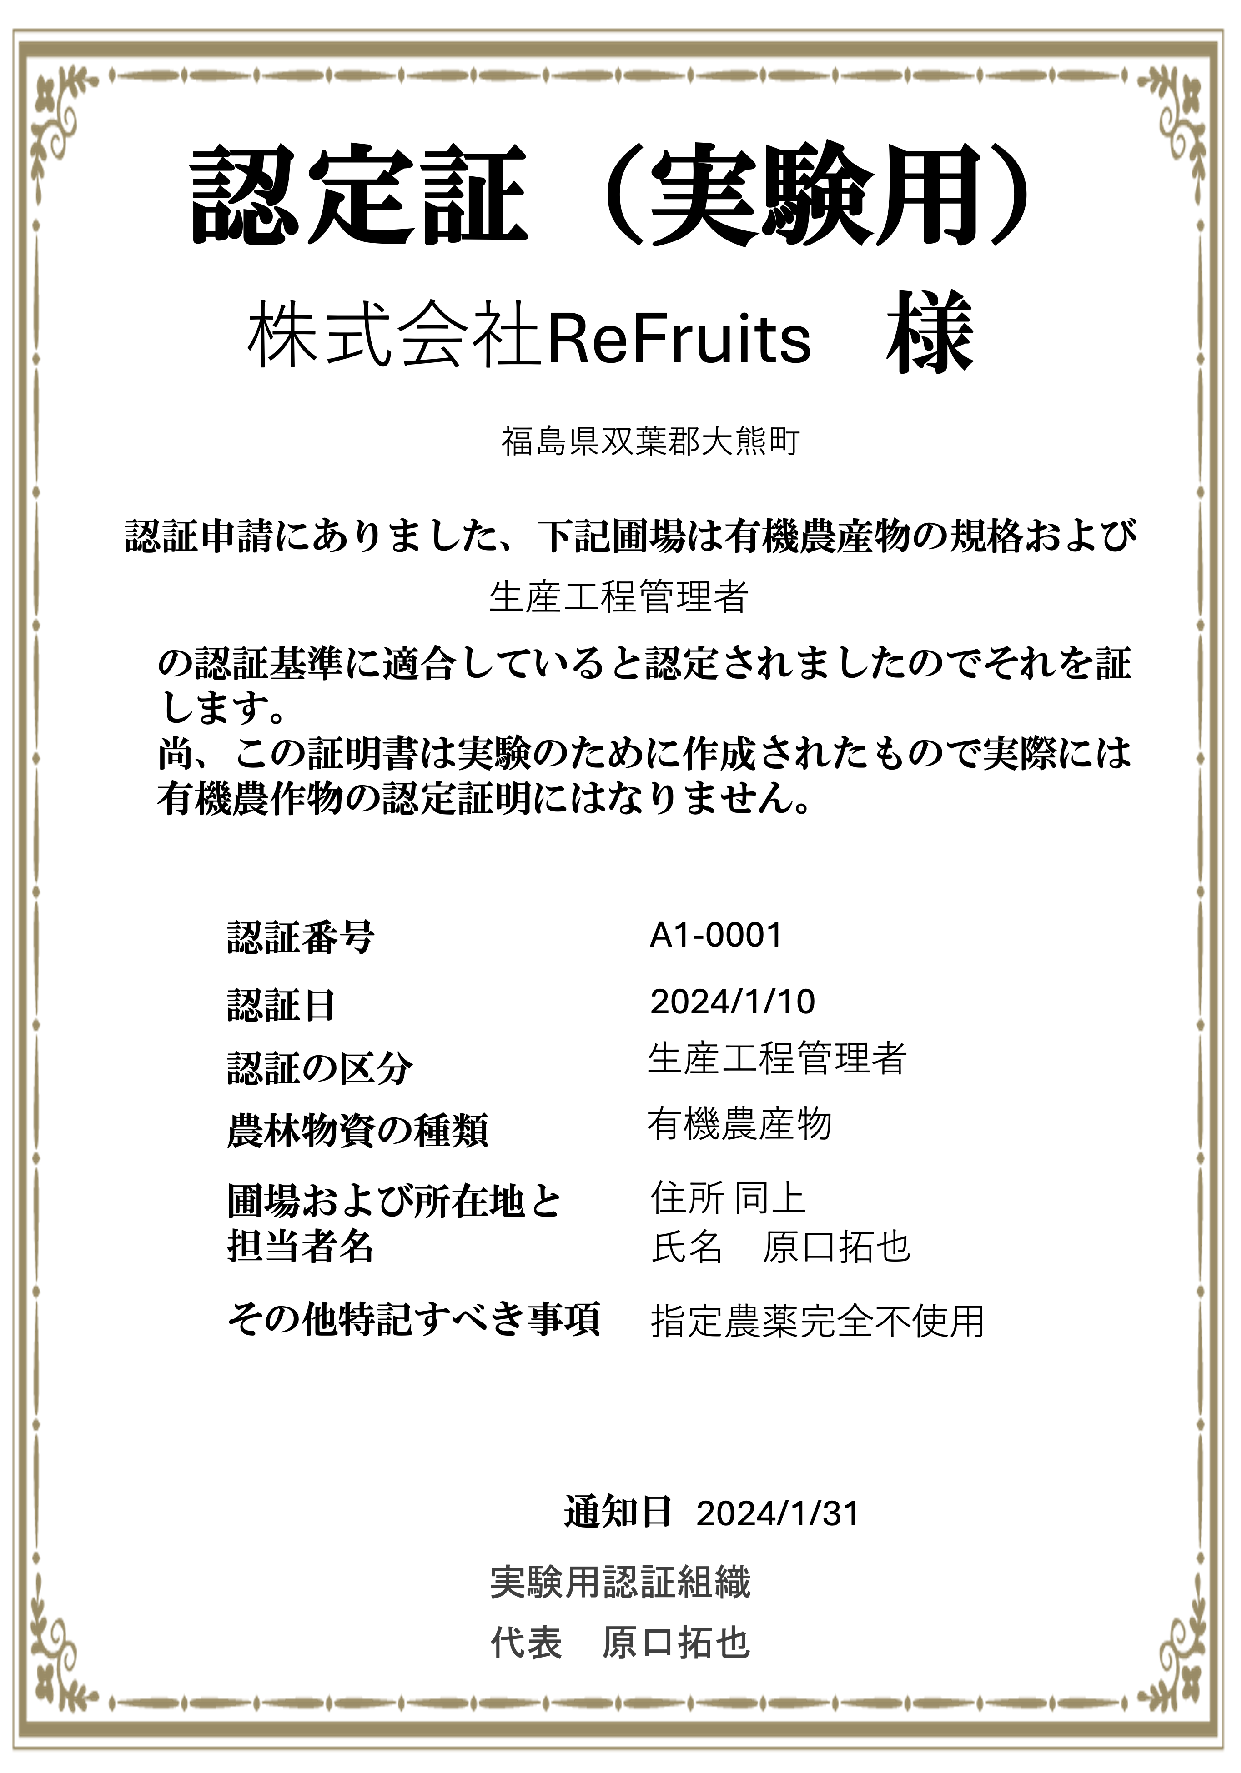
\includegraphics[width=0.8\linewidth]{Haraguchi_fig/ninnssyou.pdf}
	\caption{有機栽培の認定証}
	\label{fig:ninteisyou}
\end{figure*}

まずは,GitHub上に公開されているBlockCertsのcert-issuerを取り込み,依存関係を追加インストールを実行する.

   次に,証明書を作成するためには検証で使用する公開鍵を指定する必要があり,BloCkcertsでは検証方法を指定するのにDID(Decentralized ID) を使用する.ここではMetaMaskから秘密鍵をエクスポートし,JWK(Json WeB Key)で指定し,公開鍵へと変換する.そして,証明書を検証するのに使うために作成した公開鍵を格納するためにDIDドキュメントを作成する.こちらはWC3(World Wide Web Consortium)によって規格化されたものを使用している.



DIDを作成後,証明書に記載されている情報を記入し,作成されたjsonファイルに対してcert-issuerを使用し,指名と署名データを分散台帳上に書き込むこみ,証明書が発行される.

最終的には図\ref{fig:ninteisyou}が分散台帳上で検証が行われ,証明書は有効な証明書であることが証明される.

この証明された情報をURLをQRコードに読み込み,キウイの商品パッケージに印刷する.消費者は商品に取り込まれた情報が,正しく有機栽培認証を受けたものであることが確認が可能となる.


分散台帳によって認証を受けた場合と,既存の有機農産物認証を受けた場合の消費者の確認できる情報を表\ref{fig:hyo1}にまとめた.

\begin{table}[ht]
 	\centering
	\caption{従来手法と提案手法のステップ数の比較}
		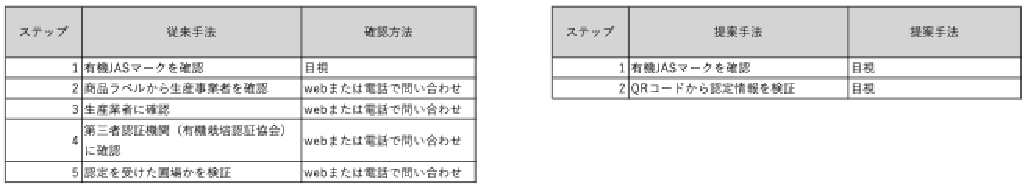
\includegraphics[width=1.0\linewidth]{Haraguchi_fig/hyou1.pdf}
	\label{fig:hyo1}
\end{table}

表\ref{fig:hyo1}より,消費者が従来の認証において,認証情報の検証を行うためには,以下の5つのステップが必要であった.

\begin{itemize}
  \item 有機JASマークを確認する(目視)
  \item 有機JASマークを確認商品ラベルから生産事業者を確認する.(電話,web等での問い合わせ)
  \item 生産業者に確認する.(電話,web等での問い合わせ)
  \item 第三者認証機関(有機栽培認証協会)に確認する.(電話,web等での問い合わせ)
  \item 認定を受けた圃場かを検証(目視)
\end{itemize}

一方,消費者が提案手法によって,認証情報の検証を行うためには,以下の2ステップが必要であった.
\begin{itemize}
  \item 有機JASマークを確認する(目視)
  \item 有機JASマークを確認商品ラベルから生産事業者を確認する.(電話,web等での問い合わせ)
\end{itemize}商品ラベルに記載のQRコードを読み取り検証する.(目視)

これにより,消費者が有機農産物の認証をする際.従来手法と提案手法ではステップ数が大きく異なることが明らかとなった.
また,消費者は,従来手法では有機JASの認証マークのみしかその作物から情報を得ることはできないが,提案手法では有機農産物の認証以外にも,農薬完全不使用などの,農家が特筆して伝える情報を確認することができた.

これについて次の章で考察を行う.

\chapter{考察}
\section{消費者から見た分散台帳技術を用いた有機農産物の評価}

消費者が有機農産物認証を受けていることを確認する方法としては,有機JASマークの確認が一般的である.しかし,このマークが偽装されている可能性を完全に排除することはできない.より確実に認証の真偽を確かめるためには,消費者が小売業者,流通業者,そして生産者に直接問い合わせて,認証情報の正確性を検証する必要がある.このプロセスは手間がかかるが,分散台帳技術を利用して認証情報をQRコードに組み込むことにより,消費者はその認証が正しいものであることを瞬時に,かつ容易に確認することが可能となる.この技術により,食品の安全性と信頼性の向上が期待される.また,QRコードから情報を読み込むとどのような農家がいつ認証を受け取り,さらに特筆すべき栽培方法が記載されているなど,認証情報以外へ情報にアクセスすることが可能となり,消費者が安心感を持ってその商品を選択する基準になることが示唆される.特に,独立した第三者によって顕彰されたトレーサビリティ情報は,消費者の信頼構築に役立つという証拠が示されている\cite{ringo}.Liuらは,中国のフジリンゴを対象とした離散的選択実験を通じて,中国の消費者の代多数が,トレーサビリティそのものよりもトレーサビリティの検証を遥かに重要視していることを明らかにした\cite{ringo}.さらに,彼らは政府による認証に最も高い価値をおき,国内または国際的な第三者認証機関による認証と比較して,政府によって認証されたリンゴに対して高価格の値段であっても支払うことを厭わなかった.これは,今回の政府による認証機関である有機農産物認証を検証して確立されているトレーサビリティであるので,今回の手法に対しても同等の結果が得られることが期待される.

\section{生産者から見た分散台帳技術を用いた有機農産物の評価}
消費者が,分散台帳の有機農産物の認証を用いることにより,購買率が増加することになれば生産者としての売り上げ増加につながるために認証を受けることに対しての重要なインセンティブになる.また,生産者にとっても有機農産物に対する認証マークのみでは伝えきれない特筆すべき栽培方法や,生産のこだわり等の情報を認証情報として分散台帳上に載せることが可能となる.これは生産者にとって他の有機農産物認証の取得者との差別化が図ることができる.また,実際に有機キウイを用いたケーススタディにおいては,有機キウイの特筆すべき栽培方法に指定農薬完全不使用と記載することで,農薬が完全に使用されていないことを明らかにした情報を載せることができ,他の商品との差別化が図ることが可能となった.一方で,この有機キウイの認証情報をQRコード上で表示する際,情報の載せるQRコードの単位はキウイ1個単位となるので,QRコードのシールの作成や,その貼り付けは生産者が担わなければならない.実際にキウイを出荷する際は,100キロ単位など大容量になることが多く,その際添付すべきシールの数は1000個を超えるため,1つの発送だけでもキウイのシールの貼り付けに対してかかる労働コストはかなりかかることがわかる.また,実際に分散台帳上へ認証情報をあげる場合,その際のブロックチェーンのシステムに関する追加コスト等がかかることを考慮する必要がある.実際に有機キウイで行ったケーススタディではイーサリアムを基盤とした分散台帳上に上げたが,その際ガス代として約300円の費用がかかった.これ認証を一つ発行するのにかかる金額で,認証情報自体は一度であるため,ガス代自体は決して高いものではない.しかし,このイーサリアムベースでの証明書の発行までに,分散台帳上での情報を第三者認証機関がデータを保持し,構築する必要があるため,そこに追加コストが発生する.そのコストが結果的に生産者に皺寄せが起こってしまうため,そこには追加のコストがかかってしまい,農家の認証取得に対するハードルを上げてしまう恐れがある.次に,トレーサビリティの観点で栽培管理情報の記録が生産者に依存していることは問題である.これはオラクル問題~\footnote[6]{オラクル問題:\url{https://ethereum.org/ja/developers/docs/oracles}}と言われ,分散台帳上に記入されるデータの信頼性や改変されていないことなどを正確に把握する必要がある.今回の有機キウイのケーススタディにおいては,キウイの栽培方法に関しては生産者自身で記入していくことになるが,そこで,農薬を使用していたとしても,使用していないと記入するだけで,改竄が容易に行われてしまうリスクがある.第三者認証協会自体も,圃場での実地調査は行うものの,その場所で指定農薬が使われていないかの確認のために,残留農薬の検査をすることなどは実施していないため,そこの部分に関しては改竄がなされるリスクが存在する.この問題は,分散台帳での提案手法以前に,有機農産物の認証方法に欠点があることが示唆される.これらの問題を踏まえて,YuらはIotデバイスと分散台帳技術を用いた認証を組み合わせたモデルを組み合わせることにより,検証者が不在のまま,トレーサビリティが提案できるモデルを提案している\cite{zyusu}.今後の議論としては記入されるデータが改竄されることなく記入される仕組み作りが必要である.

\chapter{妥当性への脅威}

\section{内的妥当性}
本研究では,分散台帳における農産物の認証の評価を自身でおこなった.実際の農産物の現場での視点との乖離が起こってしまう脅威はあるが,本研究に関しては,著者自身が農業生産者として3年間キウイ栽培に携わってきた経験があり,消費者としての側面を持つため,2つの視点で手法に対しての現実的な考察を行った.生産に関しては自信が栽培を行っていることに加え,全国の農業従事者,農業生産事業者へ30件以上伺い,農業生産や認証制度におけるヒヤリングを行ってきた.また,有機農産物の認証制度に関しても,和歌山有機栽培認証協会へ伺い,ヒヤリングを行ってきた.このように,現実に即した著者本人の経験と,ヒヤリングを重ねて行ったため,実験の手法が大きく課題から外れる危険性は少ないと考えられる.また,本研究における認証の確認をするために,消費者が信頼性を持った形で農産物認証を検証する手法としてBlockCertsを用いた.この認証手法は,DIDでの署名による認証を,改竄されない形での認証を可能とするため,信頼性を持った形で農産物における認証を可能としている.紙や従来のデータ管理であまた,BlockCerts実態がW3Cにおいて標準規格と定められているので,分散台帳による認証プロセスが信頼性を欠く可能性は低い.

\section{外的妥当性}
今回は有機キウイにおける有機農産物認証のケーススタディを行い,実際の栽培方法に近い情報を取り扱ったため,他の農産物においても同様の結果が得られることが考えられる.今回の有機キウイを用いたケーススタディにおいては,キウイの栽培に関しての生産から販売までの認証におけるトレーサビリティを詳細に記入した.これをトマト栽培,米,きゅうり栽培などの他の作物に転用した場合も同じような手順で分散台帳を用いた認証をとることが可能となる.その際,その作物はどの単位で販売されているかについて考慮する必要がある.例えば,トマトにおいてはパックでの販売がなされている場合においてはパック単位にQRコードを紐づける必要がある.米などであれば,パッケージ化された袋単位,きゅうりであれば1本単位などである.ただし,これらは商品販売の最小単位に情報を紐づけるものであり,本研究における脅威となるものではない.また,農作物だけでなく,食品業界全体で,トレーサビリティとその信頼性は重要な概念となるため,工食品や水産物など食品業界全体に応用できる可能性がある.水産加工品の認証制度においても,基本的に発生するステークホルダーは生産者,第三者認証協会,消費者と同じであるため,分散台帳を用いて認証を行うまでのステップで変更になることはないと考えられる.

\chapter{おわりに}
本研究では,農産物の認証とそのトレーサビリティについて,分散台帳を用いたシステム設計とその評価を提案し,有機農産物におけるケーススタディによってその課題と可能性に関して評価した.本研究の目的は,有機農産物の認証に関して,信頼性の観点,食品情報の透明性を向上することである.その手法として,今回は分散台帳を用いて有機農産物の認証を行った.そして,その認証システムに関して,消費者が農産物認証の検証を行う際のステップ数の比較を行った.その結果,従来手法では5つのステップ数がかかっていたのを提案手法では2つのステップ数で確認できることがわかった.また,提案手法では生産者が特筆したい栽培方法等を分散台帳上に記載することが可能となり,消費者が有機農産物認証を購入するための重要なインセンティブとなった.

\chapter*{謝辞}
本研究を進めるにあたり多くの方々に,御指導,御協力,御支援を賜わりました.ここに,御世話になった方々への感謝の意を記させて頂きます.
はじめに,指導教員である和歌山大学システム工学部伊原彰紀教授に対し,厚く御礼申し上げます.大学を一度休学し,研究分野とは全く異なる活動をしていたにもかかわらず,その活動に理解を示してくださったり,活動分野での研究の可能性を提示していただいたり多くの御指導を賜りました.先生の御尽力に敬意を表し,心より感謝いたします.
次に,株式会社サイバーリンクス様には,研究方針に関する客観的な意見やデータ収集の実装方法など研究面において多くの御指導,御協力,御助言を頂きました.お忙しい中,研究に関する相談に乗って頂き,貴重なご意見を頂いたことを特に感謝いたします.
また,和歌山有機認証協会様には,有機農産物の認証の現状,課題,可能性に関してのご意見,御助言を頂きました.心より感謝いたします.
和歌山大学ソーシャルソフトウェア工学研究室の方々には,研究に関する客観的な御意見や御協力を常日頃から数多く頂きました.研究活動だけでなく,大学生活においても大変お世話になりました.また,このコロナ禍において,満足に学業を行うことができなかった中,研究室の方々との日常での充実や日々切磋琢磨し合う同期の仲間がいたことは,研究活動を進める上で大きな支えとなりました.心より感謝いたします.
最後になりましたが,日頃から暖かく見守り,支えてくださった家族に心より深く感謝いたします.



%%%%%%%%%%%%%%%%%%%%%%%%%%%%%%%%%%%%%%%%%%%%%%%%%%%%%%%%%%%%%%%%%%%%%%%%

%%
%% 謝辞
%%
%% \begin{acknowledgements}
%% 感謝します.
%% \end{acknowledgements}

%%%%%%%%%%%%%%%%%%%%%%%%%%%%%%%%%%%%%%%%%%%%%%%%%%%%%%%%%%%%%%%%%%%%%%%%

%%
%% 参考文献
%%
\bibliographystyle{junsrt}
\bibliography{Haraguchi}

%%%%%%%%%%%%%%%%%%%%%%%%%%%%%%%%%%%%%%%%%%%%%%%%%%%%%%%%%%%%%%%%%%%%%%%%

%%
%% 付録
%%
% \appendix
% 
% \chapter{サンプルプログラム}
% 
% プログラムリストや実行結果など,本論を補足する上で必要と思われるものが
% あれば付録として付ける.
% 
% {
% \footnotesize
% \begin{verbatim}
% #include <stdio.h>
% int main(void)
% {
%     printf("Hello, World!\n");
%     return 0;
% }
% \end{verbatim}
% }

%%%%%%%%%%%%%%%%%%%%%%%%%%%%%%%%%%%%%%%%%%%%%%%%%%%%%%%%%%%%%%%%%%%%%%%%

\end{document}
